% Analítica Predictiva y Prescriptiva · TIC-60286 · Semana 2
% Vigilar el entorno con datos alternativos
% Compilar: pdflatex week-02.tex (dos veces)
%
% Plan de los 90 minutos
%   0–5    Dónde vamos (láminas 2–3)
%   5–20   El paper: Yelp y la economía local (láminas 4–8)
%  20–65   La aplicación: MAREA, la regla, la matriz, el giro (láminas 9–21)
%  65–70   Puente: el task 2 (lámina 22)
%  70–90   Cierre: las fichas del task 1 (lámina 23)
%
% Las cifras de MAREA son las del primer informe trimestral (III trimestre de 2026).
% figures/marea_senales.pdf es la figura del informe; cámbiala por la edición vigente.
% Las figuras del Club y de la matriz salen de datasets/week-02/_generar_entorno_latitud.R.
% TODO: la lámina 15 trae tres hechos de ejemplo; reemplázalos por hechos reales de la semana.

\documentclass{beamer}
\input{../../_beamer/preambulo_app.tex}
\semana{2}{Vigilar el entorno con datos alternativos}

\begin{document}

%%=================================================
%% Primer slide
\begin{frame}
\titlepage
\end{frame}

%% ====================================================== 0. DÓNDE VAMOS (0–5)
\begin{frame}{Dónde vamos}
\begin{columns}[T]
\begin{column}{0.5\textwidth}
\textbf{La semana pasada:} la ficha de la pregunta y la posición preliminar, selladas. Se discuten hoy, en el cierre.

\medskip
\textbf{Hoy, la pieza 2 del expediente:} lo que pasa afuera. Una tabla de hechos con fuente, una matriz de influencia y las dos incertidumbres que armarán los escenarios de la semana 7.
\end{column}
\begin{column}{0.5\textwidth}
\begin{block}{La sesión}
\begin{enumerate}
  \item El paper: reseñas de Yelp que miden la economía local antes que la estadística.
  \item MAREA: tres señales para Cali.
  \item La regla de la semana con tres hechos (uno no pasa).
  \item La matriz, en vivo.
  \item Cierre: sus fichas.
\end{enumerate}
\end{block}
\end{column}
\end{columns}
\end{frame}

\begin{frame}{Antes de empezar}
\parada{chat}{¿Qué señal del entorno te preocupa más para la decisión de Latitud? Una línea. Leemos cinco.}
\end{frame}

\seccion{El paper: Yelp y la economía local}
%% ====================================================== 1. EL PAPER (5–20)
\begin{frame}{Medir la economía local antes que la estadística}{Glaeser, Kim y Luca (2017), NBER}
\begin{columns}[T]
\begin{column}{0.5\textwidth}
\textbf{Qué investigaron.} Si los datos de Yelp (negocios listados y reseñas) permiten medir la actividad económica de una zona \emph{ahora}, en lugar de esperar las cifras oficiales.

\medskip
\textbf{El contexto.} Las estadísticas de establecimientos por zona en Estados Unidos (\emph{County Business Patterns}) llegan con años de rezago y para áreas gruesas. Un alcalde, un banco o una cadena deciden sin saber qué pasó el trimestre pasado en su barrio.
\end{column}
\begin{column}{0.5\textwidth}
\textbf{Qué datos y cómo.}
\begin{itemize}
  \item Negocios y reseñas de Yelp, por código postal y por sector (restaurantes aparte).
  \item Cruzados con los conteos oficiales de establecimientos.
  \item Un modelo de \emph{nowcasting}: con Yelp de hoy y de ayer, predecir el cambio oficial que todavía no se publica, probado en una muestra reservada.
\end{itemize}
\end{column}
\end{columns}
\end{frame}

\begin{frame}{Qué encontraron}
\begin{itemize}\itemsep6pt
  \item Los cambios en los conteos de negocios y restaurantes de Yelp \textbf{anticipan} los cambios de los conteos oficiales.
  \item Un modelo con Yelp actual y rezagado explica cerca del \textbf{29\,\%} de lo que los datos oficiales viejos no alcanzan a explicar, en la muestra reservada.
  \item La señal es mejor donde Yelp ve más: zonas \textbf{densas, con más ingreso y más educación}. Donde la plataforma cubre poco, mide poco.
\end{itemize}
\medskip
\importa{Un dato alternativo mide un sustituto de lo que quieres, con un sesgo de cobertura que hay que conocer. Sirve cuando sabes a quién no ve.}
\end{frame}

\begin{frame}{Dos primos del mismo método}
\begin{columns}[T]
\begin{column}{0.5\textwidth}
\begin{block}{Luces nocturnas}
Henderson, Storeygard y Weil (2012, \emph{American Economic Review}). Imágenes satelitales de la luz nocturna, 1992--2008, para medir el crecimiento económico donde las estadísticas son débiles o no existen. La luz y el producto crecen juntos, con una elasticidad cercana a 0.3; sirve para países y regiones, no para una cuadra.
\end{block}
\end{column}
\begin{column}{0.5\textwidth}
\begin{block}{Celulares en Ruanda}
Blumenstock, Cadamuro y On (2015, \emph{Science}). Los registros de llamadas de un millón y medio de usuarios, más una encuesta telefónica a unos cientos de ellos, predicen la riqueza de cada persona y reproducen el mapa de pobreza del país que una encuesta nacional tarda años y millones en producir. Es el caso que cuenta Sosa Escudero.
\end{block}
\end{column}
\end{columns}
\end{frame}

\begin{frame}{Por qué importa para quien decide}
\begin{block}{Tres lecciones}
\begin{enumerate}\itemsep4pt
  \item El dato oficial es el patrón de referencia, pero llega tarde. Quien decide necesita \textbf{una lectura de hoy}, aunque sea aproximada, y saber cuánto se desvía del patrón.
  \item Todo dato alternativo tiene \textbf{un sesgo de cobertura}. Yelp ve el barrio rico; la luz ve la ciudad, no el punto de venta. Usarlo bien es saber a quién no ve.
  \item Cuando la fuente propia no existe, se construye: un monitor es una decisión de inversión, con costo y mantenimiento.
\end{enumerate}
\end{block}
\parada{el puente}{La gerencia de expansión de Latitud quiere saber cómo va el norte de Barranquilla \textbf{este mes}; el dato oficial llega en meses. ¿Qué mira mientras tanto?}
\end{frame}

\seccion{La aplicación: MAREA, la regla y la matriz}
%% ====================================================== 2. LA APLICACIÓN (20–65)
\begin{frame}{MAREA: un monitor para Cali}{Monitor de Actividad Regional con Estadísticas Alternativas}
\begin{columns}[T]
\begin{column}{0.55\textwidth}
\begin{itemize}\itemsep5pt
  \item La Cámara de Comercio de Cali necesita saber cómo le fue a la ciudad \textbf{el mes pasado}, por zonas. El dato oficial de actividad llega con meses de rezago y no baja a los barrios.
  \item Cienfi (Universidad Icesi) construyó un monitor con tres señales independientes, para Cali y sus \textbf{90 Distritos Económicos Especiales}.
  \item Primer informe trimestral: III trimestre de 2026.
\end{itemize}
\end{column}
\begin{column}{0.45\textwidth}
\begin{block}{La idea}
Cada señal se compara con \textbf{su propia referencia}: 100 significa ``igual que lo esperado''. Lo que se lee no es el nivel; es la desviación frente al patrón.
\end{block}
\end{column}
\end{columns}
\end{frame}

\begin{frame}{Las tres señales}
\footnotesize
\begin{tabular}{@{}p{0.19\textwidth} p{0.29\textwidth} p{0.2\textwidth} p{0.2\textwidth}@{}}
\toprule
Señal & Qué mide & 100 significa & A quién no ve \\
\midrule
Luminosidad nocturna (satélite) & La escala de la operación urbana, por zona & La luz de las mismas fechas de 2024 y 2025 & A un negocio pequeño; a lo que pasa de día; a las noches nubladas \\
Afluencia a los establecimientos (mapas) & Cuánta gente entra frente al patrón habitual de ese lugar, esa hora y ese día & La afluencia esperada del propio establecimiento & La caja: gente no es venta \\
Flujo de reseñas (panel fijo de 75.796 establecimientos) & Reseñas nuevas entre dos cierres de mes & El flujo del mes anterior & A quien no reseña; a los sectores que nadie reseña \\
\bottomrule
\end{tabular}
\end{frame}

\begin{frame}{El III trimestre de 2026, en una figura}
\begin{center}
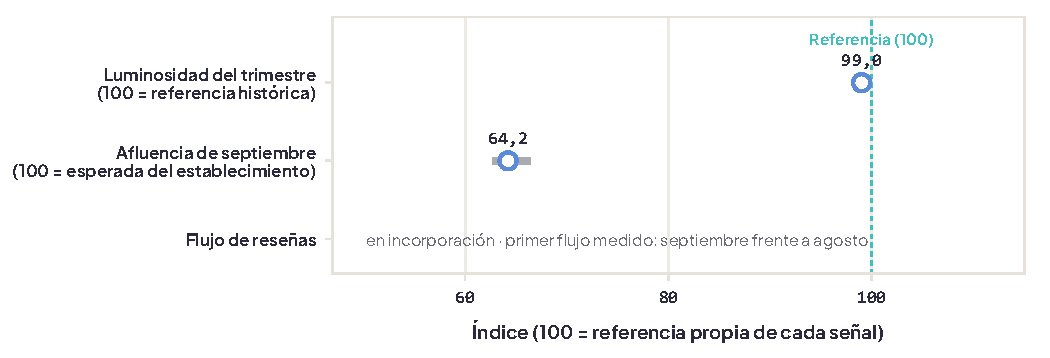
\includegraphics[width=\textwidth,height=0.72\textheight,keepaspectratio]{figures/marea_senales.pdf}
\end{center}
{\scriptsize\color{gris} Fuente: MAREA, primer informe trimestral. Luminosidad: 100 = mismas fechas de 2024 y 2025. Afluencia: 100 = la afluencia esperada del propio establecimiento para esa hora y ese día.}
\end{frame}

\begin{frame}{El III trimestre de 2026, en tres cifras}
\begin{columns}[T]
\begin{column}{0.55\textwidth}
\begin{itemize}\itemsep6pt
  \item \textbf{Luminosidad: 99.0} (intervalo 98.3 a 99.8). La ciudad opera a su escala habitual: julio por encima (101.3), agosto por debajo (97.5) tras la semana del sismo, septiembre 97.8.
  \item \textbf{Afluencia: 64.2} en septiembre. Los negocios reciben menos visitas de las que sus patrones anticipan; 3.3 puntos más que la segunda mitad de agosto.
  \item \textbf{Reseñas:} el panel está construido; el primer flujo publicable sale con el cierre de septiembre.
\end{itemize}
\end{column}
\begin{column}{0.45\textwidth}
\importa{\textbf{El contraste es territorial:} el Norte emite más luz que su patrón y el Sur registra la menor afluencia de la ciudad. Dos señales independientes que no dicen lo mismo son más útiles que una sola que lo dice todo.}
\end{column}
\end{columns}
\end{frame}

\begin{frame}{Leer una señal: la semana del sismo}
\begin{itemize}\itemsep6pt
  \item Agosto perdió su principal evento: el Festival Petronio Álvarez se suspendió tras el sismo y la agenda cultural se corrió al último trimestre.
  \item La luminosidad lo registró como la semana de menor luz del semestre; después regresó a su nivel.
  \item La afluencia lo registró como una caída y una recuperación lenta, con el Sur rezagado.
  \item Ninguna de las dos lo \emph{explica}; las dos lo \emph{muestran} a tiempo. La explicación la pone quien conoce la ciudad.
\end{itemize}
\medskip
\importa{Un monitor no reemplaza el criterio: lo alimenta. La lectura ``el Sur se recupera despacio'' es un hecho; ``por el sismo'' es una hipótesis que se verifica con otra fuente.}
\end{frame}

\begin{frame}{Lo que cada señal no ve}
\parada{chat}{Latitud quiere saber cómo va el norte de Barranquilla este mes. De las fuentes alternativas de la teoría (luces, afluencia, reseñas, búsquedas, arriendos, empleo, movilidad), ¿cuál usarías y a quién no vería?}
\medskip
\begin{itemize}
  \item La luz no ve un punto de venta: mide la cuadra de noche.
  \item La afluencia ve gente, no ventas.
  \item Las reseñas ven a quien reseña: los extremos.
  \item Los arriendos pedidos no son los pactados.
\end{itemize}
\end{frame}

\begin{frame}{Del dato al criterio: la regla de la semana}
\small
\textbf{Señal:} un hecho, una fuente. \textbf{Tendencia:} dos o más fuentes. \textbf{Impulsor:} dos o más fuentes y una magnitud económica. \textbf{Ruido:} sin fuente o sin hecho.
\medskip

% TODO: reemplazar por tres hechos reales de la semana, con su enlace. El tercero es el error sembrado.
\footnotesize
\begin{tabular}{@{}p{0.54\textwidth} p{0.19\textwidth} p{0.17\textwidth}@{}}
\toprule
Hecho (ejemplos para el ejercicio) & Fuentes & ¿Qué es? \\
\midrule
Los precios mayoristas de los alimentos suben a una tasa de dos dígitos por segundo año consecutivo & DANE; Fenalco & \\
Dos informes gremiales del año registran una caída de las visitas a los puntos de venta de conveniencia en Bogotá & Dos informes & \\
``Barranquilla es la nueva capital del comercio de conveniencia'' & Una publicación en redes, sin enlace & \\
\bottomrule
\end{tabular}
\medskip

\parada{chat}{Clasifica los tres. ¿Cuál no pasa, y por qué?}
\end{frame}

\begin{frame}{La prueba de la fuente, en sesenta segundos}
\begin{enumerate}\itemsep6pt
  \item Abrir el enlace. Si no hay enlace, el hecho no existe.
  \item Mirar la fecha. Un hecho de 2021 no es una señal de 2026.
  \item Mirar quién publica y qué gana publicándolo.
  \item Encontrar la frase exacta que respalda el hecho. Quince palabras bastan.
  \item Si dos notas citan el mismo informe, es \textbf{una} fuente.
\end{enumerate}
\medskip
\begin{exampleblock}{En el task}
Numeran las filas de su tabla, tiran un dado tres veces y hacen esta prueba con las tres filas que salgan. En el cierre de la sesión 3 yo la hago con una fila de un equipo cualquiera.
\end{exampleblock}
\end{frame}

\begin{frame}{La matriz, en vivo}
\begin{columns}[T]
\begin{column}{0.5\textwidth}
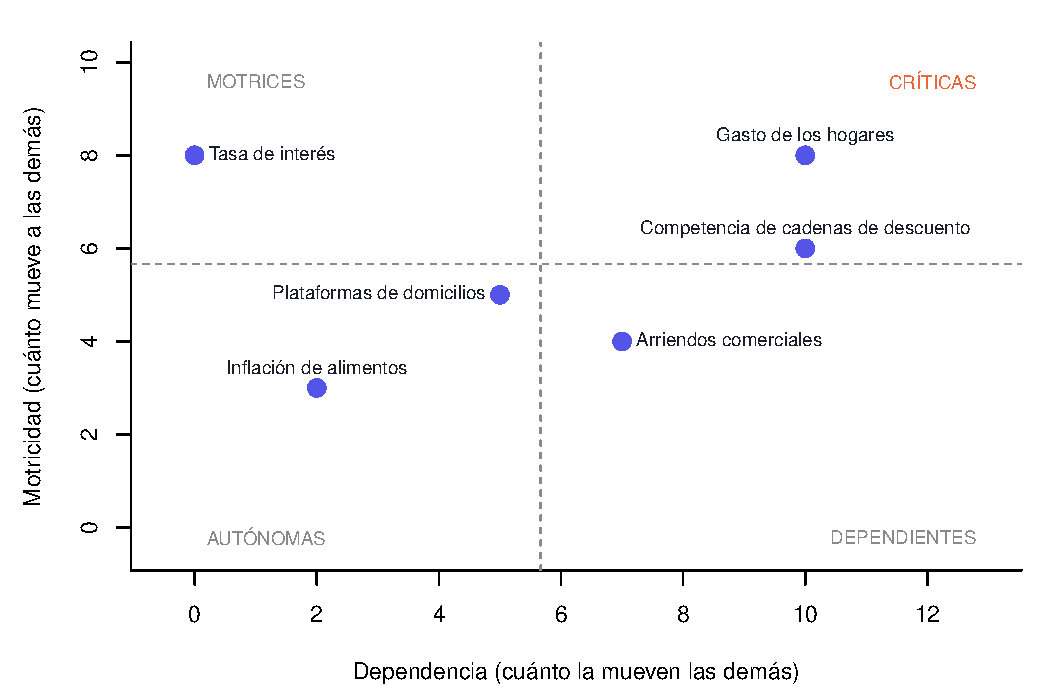
\includegraphics[width=\textwidth]{figures/matriz_plano.pdf}
\end{column}
\begin{column}{0.5\textwidth}
\small
Seis variables del entorno de Latitud: inflación de alimentos, arriendos comerciales, gasto de los hogares, competencia de cadenas de descuento, tasa de interés, plataformas de domicilios.

\medskip
\parada{encuesta}{Tres celdas las vota la sala, de 0 a 3: ¿cuánto influye la tasa de interés sobre el gasto de los hogares? ¿Y el gasto sobre los arriendos? ¿Y las plataformas sobre la competencia?}

Con las sumas de filas (motricidad) y de columnas (dependencia), cada variable cae en una zona del plano.
\end{column}
\end{columns}
\end{frame}

\begin{frame}{Leer el plano}
\begin{columns}[T]
\begin{column}{0.5\textwidth}
\begin{itemize}\itemsep5pt
  \item \textbf{Motrices:} mueven y nadie las mueve. La tasa de interés.
  \item \textbf{Críticas:} mueven y son movidas; amplifican. El gasto de los hogares y la competencia de cadenas de descuento.
  \item \textbf{Dependientes:} son resultado. Los arriendos.
  \item \textbf{Autónomas:} van por su cuenta; se vigilan. La inflación de alimentos, las plataformas.
\end{itemize}
\end{column}
\begin{column}{0.5\textwidth}
\importa{Las candidatas a ejes de escenario salen de las motrices y las críticas. De ellas, las \textbf{dos más inciertas} a tres años. Dos equipos con las mismas variables pueden llegar a planos distintos: la diferencia es criterio, y se discute.}
\end{column}
\end{columns}
\end{frame}

\begin{frame}{Reducible o irreducible}
\begin{columns}[T]
\begin{column}{0.5\textwidth}
\begin{exampleblock}{Reducible: se compra con datos o con un piloto}
Cuánto vendería un local en Barranquilla. Qué riesgo de cierre tiene un perfil de punto de venta. Cuánto responde el Club a la inversión digital. \textbf{Semanas 3 a 6.}
\end{exampleblock}
\end{column}
\begin{column}{0.5\textwidth}
\begin{alertblock}{Irreducible: se administra con escenarios}
La inflación de alimentos en 2028. La tasa de interés en dos años. Si una cadena extranjera entra. \textbf{Semana 7.}
\end{alertblock}
\end{column}
\end{columns}
\medskip
Las dos incertidumbres críticas del task deben ser irreducibles. Si una resulta reducible, no va a los escenarios: va a la lista de datos por conseguir.
\end{frame}

\begin{frame}{Noticia de última hora}
\parada{el giro}{``El arriendo comercial pedido en el norte de Barranquilla subió 18\,\% en 2026, según un portal inmobiliario; la Cámara de Comercio había reportado 12\,\% en 2025.'' \\[4pt] ¿Señal, tendencia o impulsor? ¿Riesgo u oportunidad? ¿A qué alternativa afecta más: la tienda, el Club, el piloto o esperar?}
\medskip
\begin{itemize}
  \item Dos fuentes, una magnitud: impulsor.
  \item Riesgo para la tienda y para el piloto; apenas afecta al Club.
  \item Y una pregunta para la semana 6: ¿cuánto tiene que vender la tienda para pagar ese arriendo?
\end{itemize}
\end{frame}

\begin{frame}{Lo que importa}
\importa{%
\begin{enumerate}\itemsep5pt
  \item \textbf{Vigilar es contar fuentes.} Una vez, señal; dos, tendencia; dos y una cifra, impulsor. La regla te protege del titular que nadie más reporta.
  \item \textbf{Todo dato alternativo es un sustituto} con un sesgo de cobertura. Sirve cuando sabes a quién no ve.
  \item \textbf{La matriz separa lo que mueve de lo que es movido.} De las motrices y las críticas, las dos más inciertas son los ejes de los escenarios.
\end{enumerate}}
\end{frame}

\seccion{El task y el cierre}
%% ====================================================== 3. PUENTE (65–70)
\begin{frame}{Task 2: vigilar el entorno de Latitud}
\begin{columns}[T]
\begin{column}{0.55\textwidth}
\textbf{Qué se entrega} (una página, en equipo, antes de la sesión 3):
\begin{itemize}
  \item la tabla de vigilancia: máximo doce hechos, cada uno con enlace, fecha, cifra, tipo, dirección y alternativa; tres filas verificadas con la prueba del dado;
  \item la matriz de influencia llenada a mano, con el texto que exporta el widget y el plano;
  \item las dos incertidumbres críticas, irreducibles, con una línea cada una.
\end{itemize}
\end{column}
\begin{column}{0.45\textwidth}
\begin{exampleblock}{En el cierre de la sesión 3}
Dos equipos al azar muestran su matriz; comparamos por qué difieren. Y la prueba de la fuente, en vivo, con una fila de un equipo cualquiera.
\end{exampleblock}
\end{column}
\end{columns}
\end{frame}

%% ====================================================== 4. CIERRE (70–90)
\begin{frame}{Cierre: la ficha de Latitud}
\begin{enumerate}\itemsep8pt
  \item \textbf{Dos equipos al azar, dos minutos cada uno} (6 minutos). El expositor también al azar. Muestran su ficha: la decisión, las alternativas, el criterio, el costo de cada error.
  \item \textbf{La pregunta} (8 minutos): ¿qué dato cambiaría su decisión y cuánto costaría conseguirlo? ¿Ese dato es reducible o irreducible?
  \item \textbf{Tu organización} (4 minutos): tres personas cuentan la decisión que hoy se toma ``con el pronóstico'' y cuál de los dos errores es más caro.
  \item \textbf{Dudas} (2 minutos): la entrega del task 2 y el widget de la matriz.
\end{enumerate}
\end{frame}

\begin{frame}{Referencias}
\small
\begin{itemize}\itemsep4pt
  \item Glaeser, E. L., Kim, H. y Luca, M. (2017). Nowcasting the local economy: using Yelp data to measure economic activity. \emph{NBER Working Paper} 24010.
  \item Henderson, J. V., Storeygard, A. y Weil, D. N. (2012). Measuring economic growth from outer space. \emph{American Economic Review}, 102(2), 994--1028.
  \item Blumenstock, J., Cadamuro, G. y On, R. (2015). Predicting poverty and wealth from mobile phone metadata. \emph{Science}, 350(6264), 1073--1076.
  \item Cienfi, Universidad Icesi (2026). \emph{MAREA, III trimestre de 2026: primer informe trimestral}.
  \item Sosa Escudero, W. (2019). \emph{Big data}. Siglo XXI. El apartado sobre Ruanda.
\end{itemize}
\end{frame}

\end{document}
